\documentclass[12pt]{article}
\usepackage[utf8]{inputenc}
\usepackage[spanish]{babel}
\usepackage{graphicx}
\usepackage{float} 
\usepackage[nottoc,notlot,notlof]{tocbibind} % Hace que se agregen las referencias al indice
%Paquetes para el código
\usepackage{xcolor}
\usepackage{listings}
%Estilo personalizados para el código
\definecolor{mGreen}{rgb}{0,0.6,0}
\definecolor{mGray}{rgb}{0.5,0.5,0.5}
\definecolor{mPurple}{rgb}{0.58,0,0.82}
\definecolor{backgroundColour}{rgb}{0.95,0.95,0.92}
\lstdefinestyle{CStyle}{
	backgroundcolor=\color{backgroundColour},   
	commentstyle=\color{mGreen},
	keywordstyle=\color{magenta},
	numberstyle=\tiny\color{mGray},
	stringstyle=\color{mPurple},
	basicstyle=\footnotesize,
	breakatwhitespace=false,         
	breaklines=true,                 
	captionpos=b,                    
	keepspaces=true,                 
	numbers=left,                    
	numbersep=5pt,                  
	showspaces=false,                
	showstringspaces=false,
	showtabs=false,                  
	tabsize=2,
	language=C
}
%Para acentos y esas cosas
\lstset{literate=
	{á}{{\'a}}1 {é}{{\'e}}1 {í}{{\'i}}1 {ó}{{\'o}}1 {ú}{{\'u}}1
	{Á}{{\'A}}1 {É}{{\'E}}1 {Í}{{\'I}}1 {Ó}{{\'O}}1 {Ú}{{\'U}}1
	{à}{{\`a}}1 {è}{{\`e}}1 {ì}{{\`i}}1 {ò}{{\`o}}1 {ù}{{\`u}}1
	{À}{{\`A}}1 {È}{{\'E}}1 {Ì}{{\`I}}1 {Ò}{{\`O}}1 {Ù}{{\`U}}1
	{ä}{{\"a}}1 {ë}{{\"e}}1 {ï}{{\"i}}1 {ö}{{\"o}}1 {ü}{{\"u}}1
	{Ä}{{\"A}}1 {Ë}{{\"E}}1 {Ï}{{\"I}}1 {Ö}{{\"O}}1 {Ü}{{\"U}}1
	{â}{{\^a}}1 {ê}{{\^e}}1 {î}{{\^i}}1 {ô}{{\^o}}1 {û}{{\^u}}1
	{Â}{{\^A}}1 {Ê}{{\^E}}1 {Î}{{\^I}}1 {Ô}{{\^O}}1 {Û}{{\^U}}1
	{œ}{{\oe}}1 {Œ}{{\OE}}1 {æ}{{\ae}}1 {Æ}{{\AE}}1 {ß}{{\ss}}1
	{ű}{{\H{u}}}1 {Ű}{{\H{U}}}1 {ő}{{\H{o}}}1 {Ő}{{\H{O}}}1
	{ç}{{\c c}}1 {Ç}{{\c C}}1 {ø}{{\o}}1 {å}{{\r a}}1 {Å}{{\r A}}1
	{€}{{\euro}}1 {£}{{\pounds}}1 {«}{{\guillemotleft}}1
	{»}{{\guillemotright}}1 {ñ}{{\~n}}1 {Ñ}{{\~N}}1 {¿}{{?`}}1
}
% Title Page
\title{Reporte 05A.- Transformada Rápida de Fourier}
\author{Alumno: Monroy Martos Elioth \\ Boleta: 2016630258 \\ Profesor: Gutierrez Aldana Eduardo  \\ Materia: Teoría de Comunicaciones y Señales \\ Grupo: 3CM6}
%Contenido del reporte
\begin{document}
\pagenumbering{gobble}% Remove page numbers (and reset to 1)
\maketitle
\newpage
\tableofcontents
\newpage
\pagenumbering{arabic}% Arabic page numbers (and reset to 1)
\section{Introducción}
El formato de archivos de audio digital wav (o wave), es un formato sin compresión de datos que fue desarrollado por Microsoft e IBM, es utilizado para almacenar sonidos en una computadora. Admite archivos mono y estéreos (un canal o dos respectivamente) a diversas resoluciones y velocidades de muestreo.\\ Debido a que no presenta pérdida de calidad, es comúnmente usado profesionalmente para guardar audio en CDs o DVDs. Pero tiene como desventaja, que los archivos creados bajo este formato son bastante grandes en comparación con otros formatos comprimidos como mp3 u ogg.\\ El formato de archivos wav es una variante del formato RIFF (formato de archivo para el intercambio de recursos). Un archivo en formato RIFF, empieza con una cabecera de archivo (file header) seguida de una secuencia de fragmentos de datos (data chunks). Un archivo wav comúnmente, es solo un archivo RIFF pero con una sola ''wave'' chunk, la cual esta formada por dos sub-chunks (fmt sub-chunk y data sub-chunk). A esta forma se le conoce como la forma ''canónica'' de un archivo en formato wav.\\
A continuación se presenta una lista con todos los campos que almacenan la información dentro del archivo wav:
\begin{itemize}
	\item ChunkID (4 bytes): Contiene las letras ''RIFF'' en ascii.
	\item ChunkSize (4 bytes): Es el tamaño del archivo entero menos los 8 bytes de los campos anteriores que no son contados.
	\item Format (4 bytes): Contiene las letras ''WAVE''.
	\item Subchunk1ID (4 bytes): Contiene las letras ''fmt''.
	\item Subchunk1Size (4 bytes): Contiene el tamaño del resto del subchunk que queda a partir de este número.
	\item AudioFormat (2 bytes): Regularmente almacena el número 1, si se guarda algún otro número este indica algún tipo de compresión.
	\item NumChannels (2 bytes): 1 para mono, 2 para stereo.
	\item SampleRate (4 bytes): La frecuencia de muestreo que se uso para muestrear el archivo (8000, 44100, etc).
	\item ByteRate (4 bytes): Es igual a: SampleRate*NumChannels*BitsPerSample/8.
	\item BlockAlign (2 bytes): Guarda el número de bytes por cada muestra (considerando todos los canales). Se obtiene mediante: NumChannels*BitsPerSample/8.
	\item BitsPerSampl (2 bytes): La cantidad de bits que se almacenan por muestra (8 bits, 16 bits, etc).
	\item SubChunk2ID (4 bytes): Contiene las letras ''data''.
	\item SubChunk2Size (4 bytes): Es el número de bytes de los datos, también puede considerarse como el resto del subchunk apartir de este dato.
	\item Data (tamaño del SubChunk2Size): Son los datos del sonido almacenado. 
\end{itemize}
Los campos ChunkID, ChunkSize y Format componen la cabecera del archivo. Los campos Subchunk1ID, Subchunk1Size, AudioFormat, NumChannels, SampleRate, ByteRate, BlockAlign y BitsPerSample componen el primer sub-chunk llamado fmt. Los campos Subchunk2ID, Subchunk2Size y data componen el segundo sub-chunk llamado data.\\ La figura 1 muestra de forma gráfica las cabeceras y campos antes descritos:
\begin{figure}[H]
	\centering
	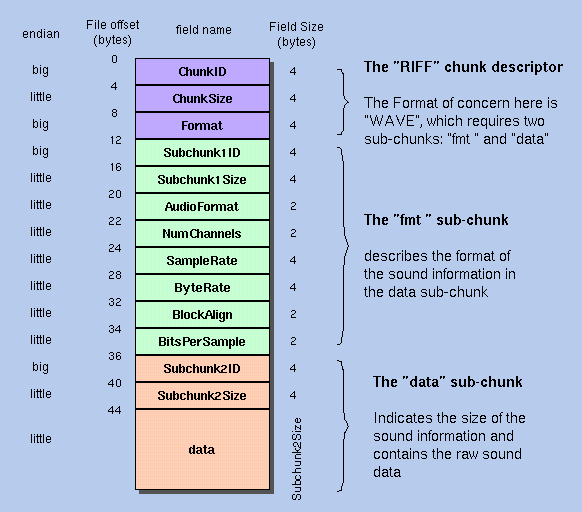
\includegraphics[scale=.7]{img/cabeceras.png}
	\caption{Campos que componen un archivo canónico wav}
	\label{fig:cabeceras}		
\end{figure}

\newpage
\section{Código}
A continuación se presenta el código del programa desarrollado que permite cambiar el volumen a un archivo en formato wav, el programa reduce el volumen del sonido a la mitad (lo cual resulta equivalente a dividir entre dos cada muestra en el archivo).\\
funciones.h:
\begin{lstlisting}[style=CStyle]
#ifndef __FUNCIONES_H__
#define __FUNCIONES_H__
	//Librerías de C
	#include <stdio.h>
	#include <stdlib.h>
	//Métodos
	void leerCabeceras(char**);
	void leerMuestras(short*);
	void dividirMuestras(short*,float);
	void escribirArchivo(short*);
	//Cabeceras
	int chunkid;
	int chunksize;
	int format;
	int subchunk1id;
	int subchunk1size;
	short audioformat;
	short numchannels;
	int samplerate;
	int byterate;
	short blockalign;
	short bitspersample;
	int subchunk2id;
	int subchunk2size;
	//Archivos
	FILE* entrada;
	FILE* salida;
	//Variables para muestras
	short muestra;
	int total_muestras;
	short headers[37];
#endif
\end{lstlisting}
\newpage
half.c:
\begin{lstlisting}[style=CStyle]
#include"funciones.h"
int main(int argc, char *argv[]){
	//Leo las cabeceras
	leerCabeceras(argv);
	//Defino variables
	total_muestras=subchunk2size/blockalign;
	short muestras[total_muestras];
	//Leo las muestras
	leerMuestras(muestras);
	//Divido el volumen a la mitad
	dividirMuestras(muestras,.5);
	//Escribo el archivo
	escribirArchivo(muestras);
}
void leerCabeceras(char ** argv){
	//Abrir archivos
	entrada = fopen(argv[1], "rb");
	salida=fopen(argv[2],"wb");
	if(!entrada) {
		perror("\nFile opening failed");
		exit(0);
	}
	fread(&chunkid,sizeof(int),1,entrada);
	fread(&chunksize,sizeof(int),1,entrada);
	fread(&format,sizeof(int),1,entrada);
	fread(&subchunk1id,sizeof(int),1,entrada);
	fread(&subchunk1size,sizeof(int),1,entrada);
	fread(&audioformat,sizeof(short),1,entrada);
	fread(&numchannels,sizeof(short),1,entrada);
	fread(&samplerate,sizeof(int),1,entrada);
	fread(&byterate,sizeof(int),1,entrada);
	fread(&blockalign,sizeof(short),1,entrada);
	fread(&bitspersample,sizeof(short),1,entrada);
	fread(&subchunk2id,sizeof(int),1,entrada);
	fread(&subchunk2size,sizeof(int),1,entrada);
}
void leerMuestras(short *muestras){
	int i=0;
	while (feof(entrada) == 0)
	{
		if(i<total_muestras){
			fread(&muestra,sizeof(short),1,entrada);
			muestras[i]=muestra;
			i++;
		}else{
			fread(&headers,sizeof(short),37,entrada);
			break;
		}
	}
}
void dividirMuestras(short *muestras, float factor){
	int i;
	for (i = 0; i < total_muestras; i++)
		{
			muestras[i]*=factor;
		}
}
void escribirArchivo(short* muestras){
	//Escribo el archivo
	fwrite(&chunkid,sizeof(int),1,salida);
	fwrite(&chunksize,sizeof(int),1,salida);
	fwrite(&format,sizeof(int),1,salida);
	fwrite(&subchunk1id,sizeof(int),1,salida);
	fwrite(&subchunk1size,sizeof(int),1,salida);
	fwrite(&audioformat,sizeof(short),1,salida);
	fwrite(&numchannels,sizeof(short),1,salida);
	fwrite(&samplerate,sizeof(int),1,salida);
	fwrite(&byterate,sizeof(int),1,salida);
	fwrite(&blockalign,sizeof(short),1,salida);
	fwrite(&bitspersample,sizeof(short),1,salida);
	fwrite(&subchunk2id,sizeof(int),1,salida);
	fwrite(&subchunk2size,sizeof(int),1,salida);
	//Ahora escribo las muestras
	int i=0;
	for(i=0;i<total_muestras;i++){
		fwrite(&muestras[i],sizeof(short),1,salida);
	}
	//Y por último los headers de goldwave
	for(i=0;i<37;i++){
		fwrite(&headers[i],sizeof(short),1,salida);
	}
}
\end{lstlisting}
\newpage
\section{Pruebas}
Para comprobar el funcionamiento de los programas se usaron los siguientes archivos wav.\\
Para realizar el filtrado mediante el producto en frecuencia, se uso como entrada para el programa de la transformada discreta de Fourier el siguiente archivo:
\begin{figure}[H]
	\centering
	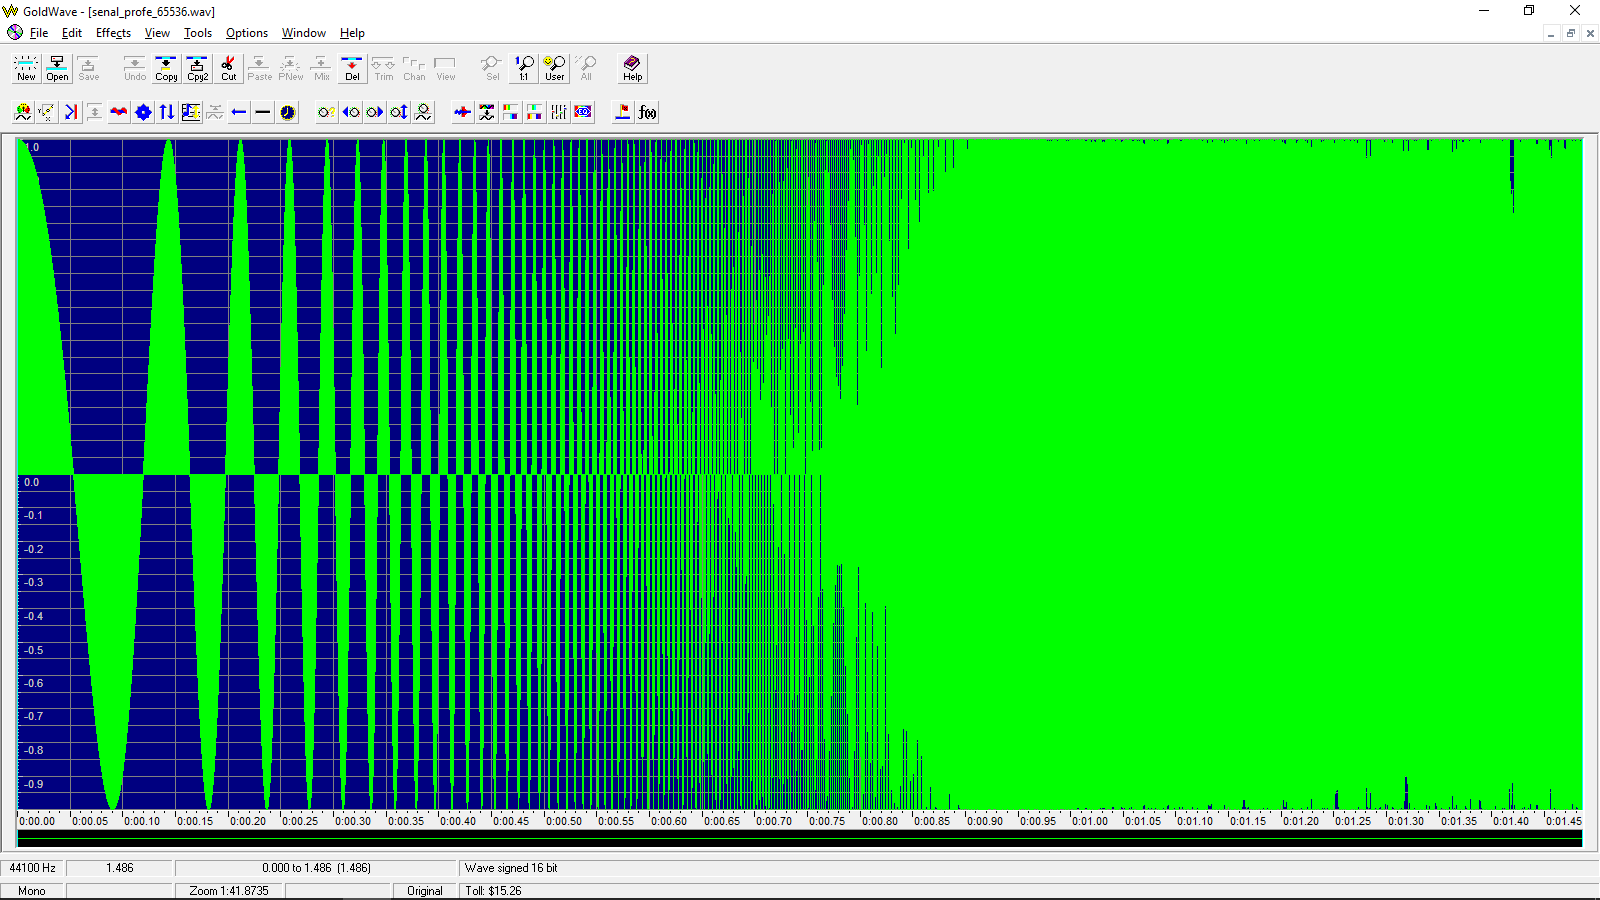
\includegraphics[scale=.35]{img/entrada.png}
	\caption{Entrada para TDF}
	\label{fig:prueba1}		
\end{figure}
El cual tiene una frecuencia de muestreo de 44100 muestras/s y una duración de .04 segundos.\\ A diferencia del archivo usado en el reporte 02A-Simulación circuito RC, donde la duración del archivo era de 1 segundo, para esta prueba se disminuyo la duración para que el número de muestras que tuviera que procesar el programa de la TDF no fuera tan grande (con esa duración y frecuencia de muestreo el total de muestras fue de 1764) y no demorara mucho tiempo ejecutándose. La función usada en el archivo fue: cos(2*pi*t*(exp(log(20)+n/N*6.6))).\newpage
La salida obtenida del programa TDF fue la siguiente:
\begin{figure}[H]
	\centering
	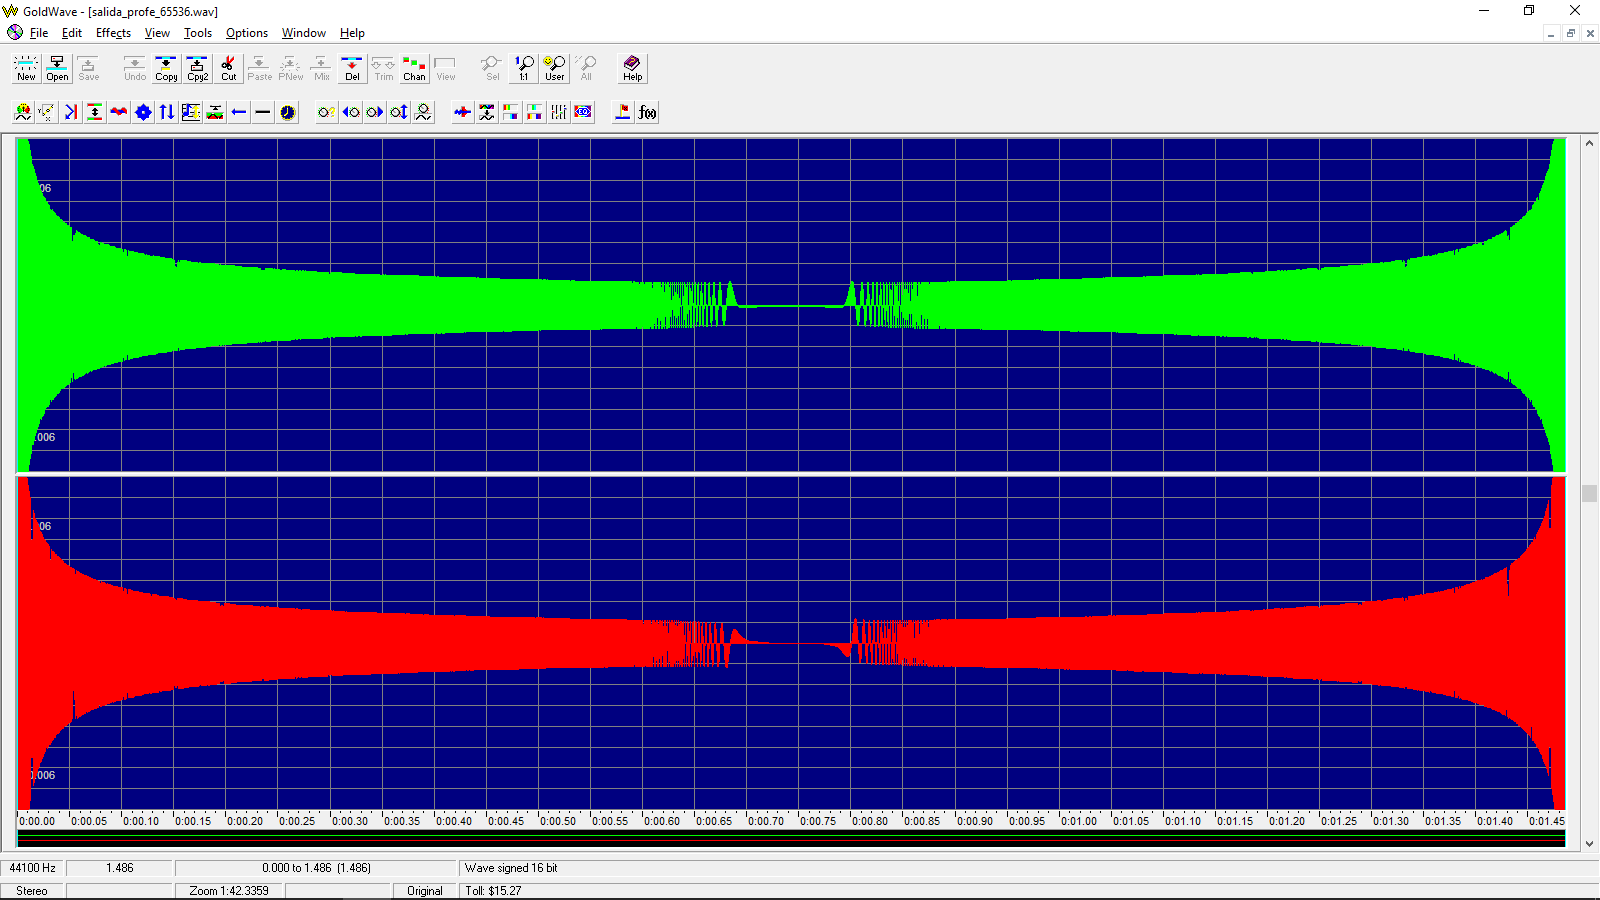
\includegraphics[scale=.3]{img/salidaTDF.png}
	\caption{Salida TDF}
	\label{fig:prueba2}		
\end{figure}
El filtro para realizar el producto se muestra en la siguiente Figura, cabe señalar que se modelo un filtro ideal con una frecuencia de corte de 1000Hz. Se creo, seleccionando solamente el canal izquierdo del archivo e ingresando la siguiente función:(step(n)-step(n-40))+step(n-(1764-40)).
\begin{figure}[H]
	\centering
	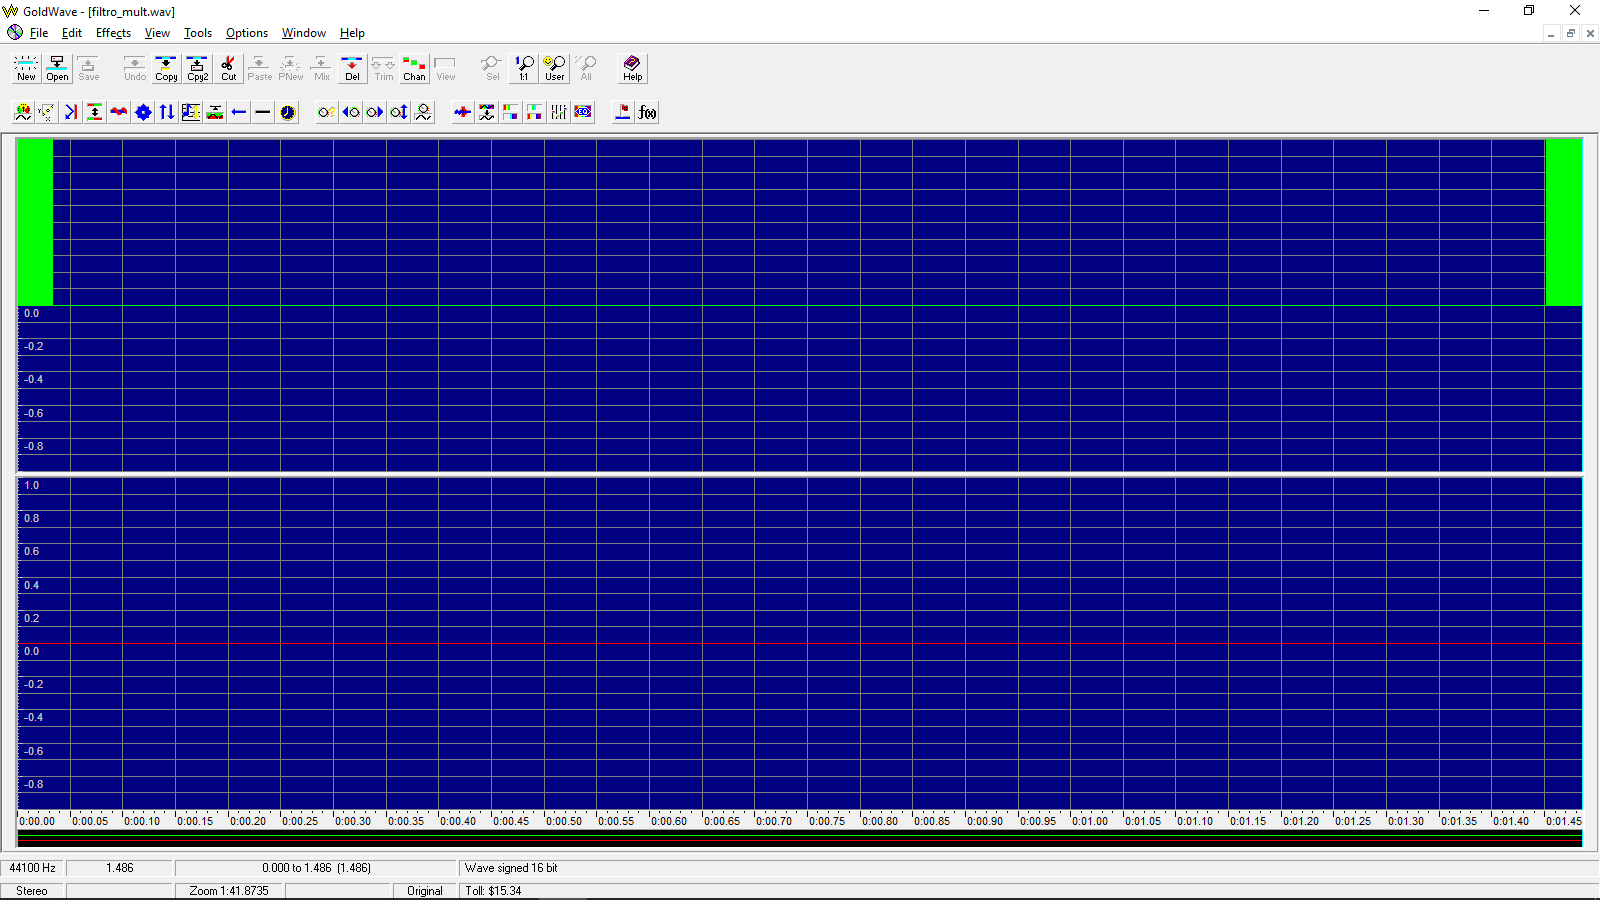
\includegraphics[scale=.3]{img/filtro.png}
	\caption{Filtro ideal con una frecuencia de corte de 1000Hz}
	\label{fig:prueba3}		
\end{figure}
Posteriormente, la salida obtenida de la TDF y el filtro fueron multiplicados usando el programa producto.exe, y se obtuvo la siguiente salida:
\begin{figure}[H]
	\centering
	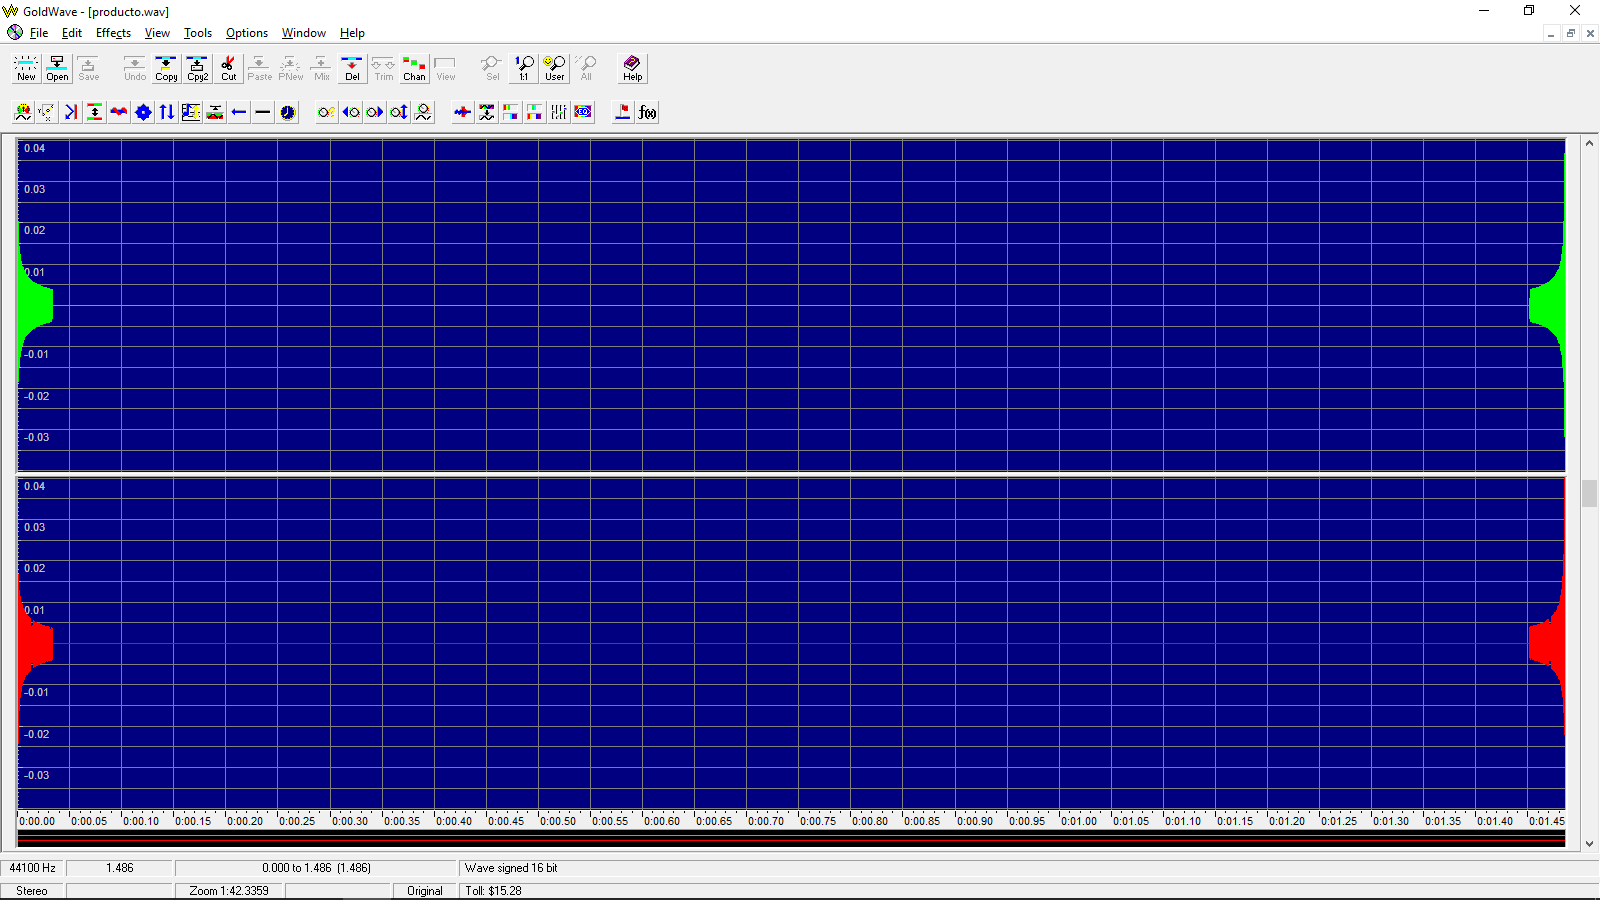
\includegraphics[scale=.35]{img/producto.png}
	\caption{Producto obtenido de multiplicar la salida de la TDF y el filtro ideal}
	\label{fig:prueba4}		
\end{figure}
A la salida obtenida por el programa del producto, finalmente fue ingresado al programa que calcula TDF Inversa, y se obtuvo la siguiente salida.
\begin{figure}[H]
	\centering
	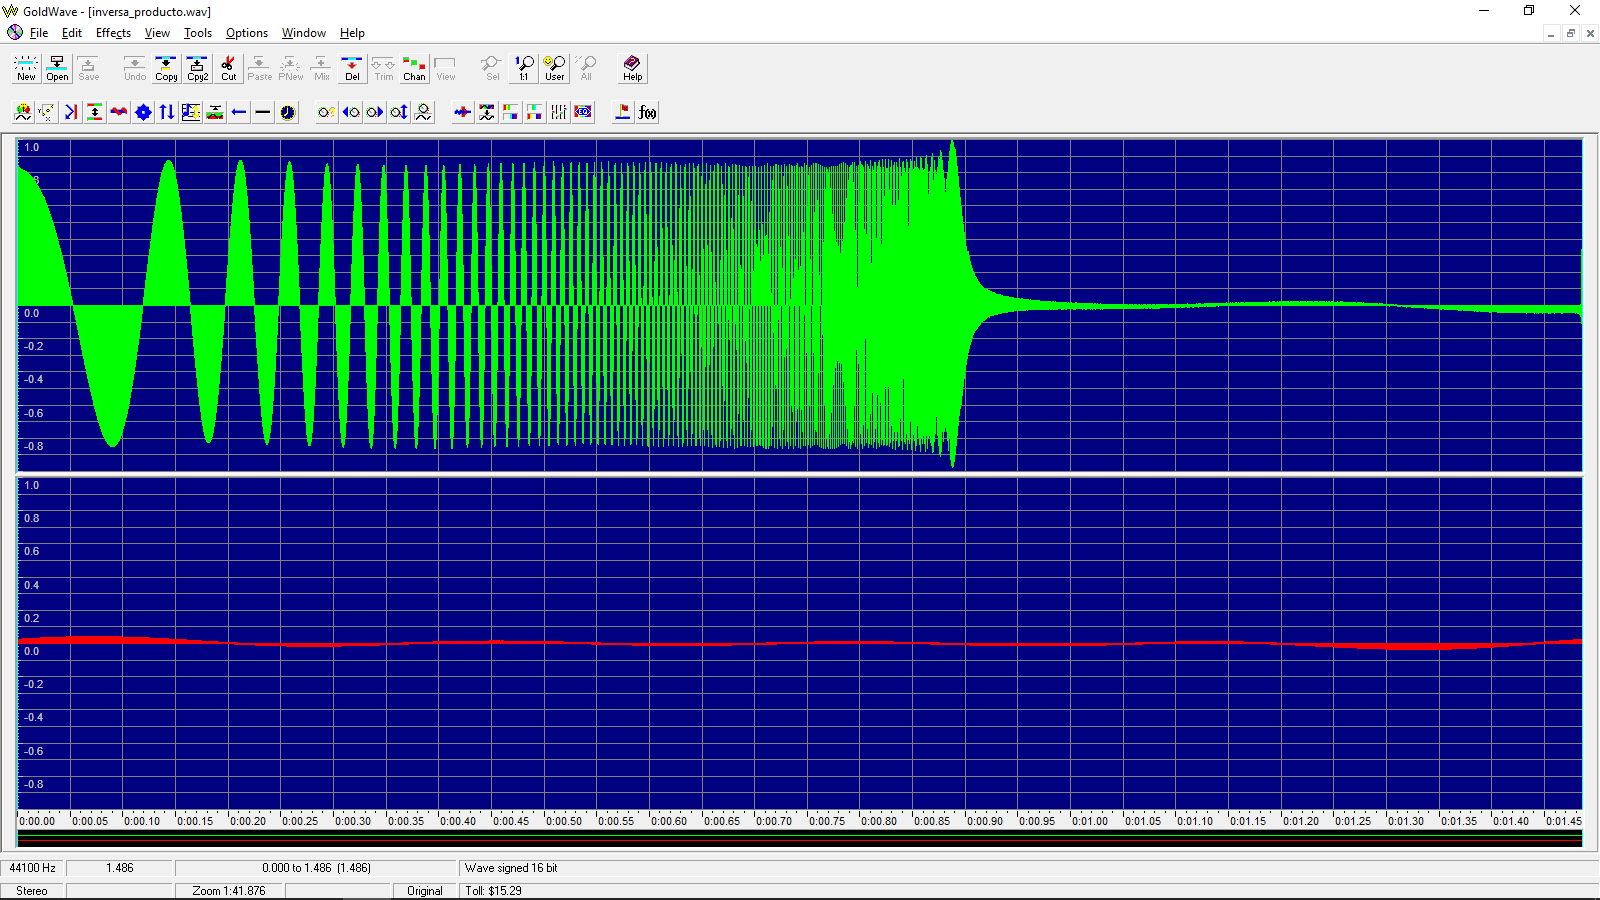
\includegraphics[scale=.32]{img/salida.png}
	\caption{Salida obtenida de la TDFI}
	\label{fig:prueba5}		
\end{figure}
Para comprobar que el resultado fuera el correcto, a la señal original de entrada se le filtro usando Goldwave, de lo cual se obtuvo la siguiente salida:
\begin{figure}[H]
	\centering
	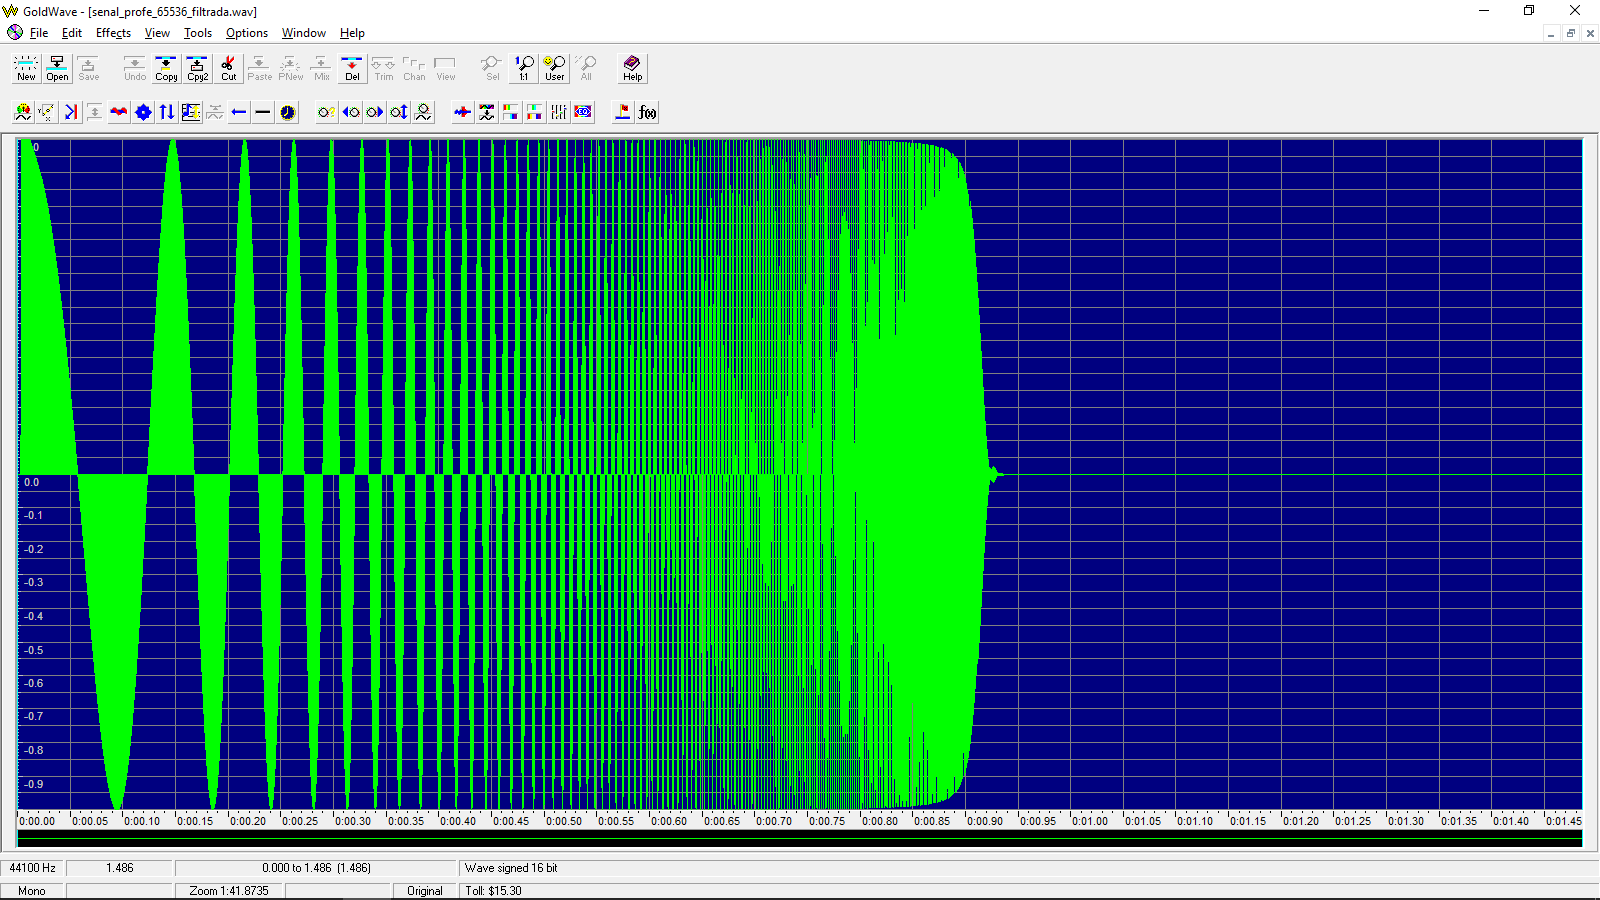
\includegraphics[scale=.32]{img/salida_goldwave.png}
	\caption{Señal original filtrada usando Goldwave}
	\label{fig:prueba6}		
\end{figure}
Como se puede observar, el filtrado realizado mediante frecuencia no es tan preciso como el hecho por Goldwave pero tiene una gran similitud con este mismo. En trabajo posterior, se repite este proceso pero usando la Transformada Rápida de Fourier (FFT).
\newpage
\subsection{Conclusiones}
	El uso de autómatas finitos deterministas y no deterministas nos permite validar que el orden en cadenas de entrada sea correcto.
	Esto tiene diversas aplicaciones, desde muy sencillas (como validar el formato de un CURP) hasta aplicaciones más complejas como realizar parte del análisis léxico de un lenguaje de entrada en un compilador.\\Los cuales nos ayudan a saber si una entrada pertenece a nuestro lenguaje o no, siendo de gran utilidad al momento de validar cadenas apartir de una expresión regular.
%Bibliografía
\bibliographystyle{ieeetr}
\bibliography{referencias}
%\cite{libro}
%\cite{rc}

\end{document}    